
% Group addresses by affiliation; use superscriptaddress for long
% author lists, or if there are many overlapping affiliations.
% For Phys. Rev. appearance, change preprint to twocolumn.
% Choose pra, prb, prc, prd, pre, prl, prstab, prstper, or rmp for journal
%  Add 'draft' option to mark overfull boxes with black boxes
%  Add 'showpacs' option to make PACS codes appear
%  Add 'showkeys' option to make keywords appear
\documentclass[aps,prd,reprint,superscriptaddress]{revtex4-1}
%\documentclass[aps,prl,preprint,superscriptaddress]{revtex4-1}
%\documentclass[aps,prl,reprint,groupedaddress]{revtex4-1}
%\usepackage{bm}
\usepackage{amsmath}
\usepackage{lineno}
\usepackage{graphicx}


%\newcommand\refsec[1]{\S\ref{sec:#1}}
%\newcommand\refeq[1]{Eq.~(\ref{eqn:#1})}
%\input{papers_packages_command._include_tex}
\newcommand\refsec[1]{\S\ref{sec:#1}}
\newcommand\refeq[1]{Eq.~(\ref{eqn:#1})}
\newcommand{\refssec}[1]{section~\ref{subsec:#1}}
\newcommand{\reffig}[1]{Fig.~\ref{fig:#1}}
%\newcommand{\apj}{ApJ}
\newcommand{\physrep}{Physics Reports}
\newcommand{\aapr}{A\&A Rev.}
\newcommand{\apjl}{ApJL}
\newcommand{\apjs}{ApJS}
\newcommand{\aap}{A\&A}
\newcommand{\mnras}{MNRAS}
%\newcommand{\prd}{Phys. Rev. D}
\newcommand{\physrev}{Phys. Rev.}
\newcommand{\physrevlett}{Phys. Rev. Lett.}
\newcommand{\jcap}{{\em JCAP }}
\newcommand{\aj}{AJ }
\bibliographystyle{apsrev4-1}

\begin{document}
\graphicspath{{images/}}

%Title of paper
\title{External priors for the next generation of CMB experiments.}

\author{Alessandro Manzotti}
\email{\href{mailto:manzotti.alessandro@gmail.com}{manzotti.alessandro@gmail.com}}
\affiliation{Department of Astronomy \& Astrophysics, University of Chicago, Chicago IL 60637}
\affiliation{Kavli Institute for Cosmological Physics, Enrico Fermi Institute, University of Chicago, Chicago, IL 60637}
\author{Scott Dodelson}

\affiliation{Department of Astronomy \& Astrophysics, University of Chicago, Chicago IL 60637}
\affiliation{Kavli Institute for Cosmological Physics, Enrico Fermi Institute, University of Chicago, Chicago, IL 60637}
\affiliation{Fermilab Center for Particle Astrophysics, Fermi National Accelerator Laboratory, Batavia, IL 60510-0500}

\date{\today}
\begin{abstract}
The next generation of cosmic microwave background (CMB) experiments can dramatically improve what we know about neutrino physics, inflation, Dark Matter and Dark Energy. 
Indeed the low level of noise, together with improved angular resolution, will allow a precise measurement of the CMB polarization anisotropies as well as an improved reconstruction of the lensing potential of high redshift large scale structure. 
Projected constraints on cosmological parameters are extremely tight, but these can be improved even further with information from external experiments. Here, we examine quantitatively, with a Fisher matrix approach, the extent to which external priors can lead to improvement in projected constraints from a CMB-Stage 4 (S4) experiment.
We find that CMB S4 constraints on neutrino masses can be limited by their degeneracies with the optical depth $\tau$ unless the largest scale at reach for CMB S4 will be large enough to constraint $\tau$ internally thought the reionization bump. To imp a $3\%$ constraint on 
\end{abstract}

\pacs{}
% insert suggested keywords - APS authors don't need to do this
\keywords{CMB, neutrinos}
\maketitle

\section{Introduction}\label{sec:intro}
Since their early stages, Cosmic Microwave Background (CMB) experiments have been crucial in our understanding of the universe. In the near future, they have the potential to maintain this important role  thanks to the unprecedented low level of noise and high resolution of their next Stage IV (S4) generation. 
Indeed, the next generation of CMB experiments (S4), now in its planning stage, will measure the E-mode polarization with almost cosmic variance limited precision together with an order of magnitude improvement in B-mode measurement and lensing reconstruction.
This new sensitivity, in particular if supported with the essential synergy with other cosmological probes, will be a a fundamental key in our understanding of dark matter, inflation, Dark Energy and neutrinos. 

Neutrinos properties can be effectively constrained with CMB measurements because they influence both the early history of the universe and the later stage of structure formation. 
In the early Universe relativistic species, like neutrinos, are the main drivers of the cosmic expansion and the expansion rate depends on their effective number $N_{\rm eff}$. This can be powerfully tested using the CMB, by comparing the sound horizon scale, obtained from the CMB peaks positions, and the Silk damping scale (see \cite{2013arXiv1309.5383A}, \cite{2013PhRvD..87h3008H} and references therein). 
S4 experiments, with their high resolution, will be able to measure the CMB power spectrum, at small scales, deeply into the damping tale, testing any possible deviations from $N_{\rm eff}=3.046$, the value predicted by the standard model.
The total mass of neutrinos, on the other hand, has a modest effect on the primary CMB because, for the range of masses allowed by recent constraints ($M_{\nu}<230$ meV from \cite{2014A&A...571A..16P}), neutrinos are still relativistic at the last scattering surface. However massive neutrinos influence the growth of structure at scales shorter than their free streaming one. Different neutrino masses consequently lead to different CMB lensing. Stage IV experiment will measure small scales temperature and polarization anisotropies with low noise, drastically improving the lensing reconstruction. This will turn into such a precise constraints of the sum of neutrino masses to get a possible hint of the hierarchical structure of the individual masses. 
Quantitatively, CMB alone will constrain the number of relativistic degree of freedom $N_{\rm eff}$ with a $1\%$ precision and the total mass of neutrinos at $45\%$ with a factor of two improvement on $M_{\nu}$ when priors from baryon acoustic oscillations (BAO) data are introduced \cite{wu:2014}. The future generation of CMB experiments will be a big step in the understanding of the neutrino sector.

As previously mentioned, CMB is also a powerful probe of the dark energy properties (see \cite{2010MNRAS.405.2639J}). The challenge for future experiments is to go beyond the, now well measured, energy density and to determine other dark energy properties.
Among these, a crucial step would be to constraint the equation of state, the ratio of pressure and energy density, looking for possible deviations from the value $w=-1$ expected in a cosmological constant scenario. 
CMB is sensitive to Dark energy because this component alters the late universe's expansion and it consequently changes the distance to the last scattering surface. Furthermore different DE models lead to a different growth of large scale structure which are tested by CMB lensing.
However, dark energy properties are strongly degenerate with other geometrical parameters like $H_{0}$ and $\Omega_{k}$. As a consequence, similarly to the neutrino sector, CMB experiments will have to rely on external prior coming from BAO and supernova experiments to fully exploit their potential.

The crucial importance of the feedback from external experiments is true not only for the dark energy and the neutrino sector. 
In the future, cosmology will hinge on the ability of combining different probes. In this regard CMB makes no exception: external priors will be fundamental to improve the already tight CMB constraints on cosmological parameters. 
In particular CMB will really benefit from experiments like large scale structure clustering and weak lensing, BAO targeted experiments, and supernovae. 
To improve the synergy between different experiments and to guide the plan of future experiments, in this work we study the dependance of CMB future constrains on the external priors assumed. For all the parameters of the standard $\Lambda$CDM plus massive neutrinos ($\Omega_c h^2,\Omega_b h^2,A_s,n_s,\tau,H_0,M_{\nu}$) together with possible non-standard extension ($N_{\rm eff},w,w_{a}$) we quantify, using a Fisher matrix approach, the CMB constraints as a function of external priors in each of the cosmological parameters.   

This paper is organized as follow: in \refsec{methods} we introduce the technique and assumptions we used to derive the effect of external priors on the CMB parameter constraints. In \refsec{results} we will describe our results and we then conclude with a discussion of them in \refsec{conclusions}.



\section{Assumptions and methods \label{sec:methods}}


To measure quantitatively the impact of external priors on the CMB ability to constrain cosmological parameters we use a Fisher matrix formalism. In this section we will quickly review  the technique and we will then present our fiducial cosmological model together with the experimental specifications we used.

As usual, we define the Fisher matrix elements as the curvature of the likelihood:
\begin{equation}
	\centering
		F_{ij} \equiv - \left\langle\frac{\partial^2 \log \mathcal{L}}{\partial \theta_i \partial \theta_j} \bigg|_{\boldsymbol{\theta} = \boldsymbol{\theta_0}}\right\rangle,
	\label{eqn:Fij_def}
\end{equation}
where $\theta_{i,j}$ represents two of the cosmological parameters and $\boldsymbol{\theta_0}$ is the fiducial values array that, by definition, maximizes the likelihood. It is important to notice that \refeq{Fij_def} implicitly assume that the likelihood is gaussian. Even if the gaussian approximation has been shown to be appropriate most of the time, exceptions exist in the literature \cite{2012JCAP...09..009W}. However, the level of accuracy needed in this work does not require a more careful modeling of the likelihoods. Moreover the gaussian approximation gets better at smaller scales (high $\ell$ in Fourier space) which, with the exception of the optical depth parameters $\tau$, is where most of the constraining power of the CMB is coming from.

For CMB experiments the Fisher matrix can be related to the power spectrum $\boldsymbol{C}_\ell$ by:
\begin{equation}
 F_{ij} = \sum_\ell \frac{2\ell+1}{2} f_{\rm sky} {\rm Tr} \left(  \boldsymbol{C}^{-1}_\ell( \theta) \frac{\partial \boldsymbol{C}_\ell}{\partial \theta_i} \boldsymbol{C}^{-1}_\ell( \theta) \frac{\partial \boldsymbol{C}_\ell}{\partial \theta_j}  \right).
 \label{eqn:Fij_def2}
 \end{equation}
In this work we constrain cosmological parameters with CMB temperature and E mode polarization together with the reconstructed lensing potential of large scale structure. For this reason, $\boldsymbol{C}_\ell$ in \refeq{Fij_def2} is:
 \begin{eqnarray}
 	\centering
		\mathbf{C}_\ell \equiv \left( \begin{array}{ccc}C_\ell^{TT} + N_\ell^{TT} & C_\ell^{TE} & C_\ell^{T\phi} \\ C_\ell^{TE} & C_\ell^{EE} + N_\ell^{EE} & 0 \\ C_\ell^{T\phi} & 0 & C_\ell^{\phi} + N_\ell^{\phi}\end{array}\right).
	\label{eqn:cov_definition}
\end{eqnarray}
Note that we are neglecting the term $C_\ell^{E\phi}$. As also noticed in previous literature \cite{wu:2014,2013PhRvD..87h3008H} this term contains very little information while adding possible numerical issues.
The terms $N_\ell^{X}$ represents the instrumental noise power of the specific experiment and will be described at the end of this section.

A lower bound on the error on the parameter $i$, marginalized over all the other parameters, $\sigma_i$, can be easily obtained as:
\begin{equation}
\sigma_i \equiv \sigma (\theta_i) \geq \sqrt{(\mathbf{ F^{-1}})_{ii}}.
\label{eqn:cramer-rao}
\end{equation}
Furthermore it is easy to introduce external priors on cosmological parameters.
Indeed we simply need to add to the Fisher matrixes elements the external priors (before we perform the matrix inversion of \refeq{cramer-rao}).
For example, a $1\%$ prior on the parameter $i$ can be added by:
\begin{equation}
F_{ii} \rightarrow F_{ii} + \frac{1}{(1\% \times  \theta_{i,\text{fid}})^2}.
\end{equation}


We chose a Fisher matrix approach because it is able to forecast future experiments performances without generating mock data and easily including external priors. 
This technique however introduces also technical difficulties. 
Indeed it is known \cite{2006astro.ph..9591A} that increasing the number of parameters used in the analysis can lead to numerical issues (see also \cite{2008PhRvD..77d2001V} in the gravitational waves context were several parameters are used).
Fisher matrix indeed can become ill-conditioned: a small change in the fisher matrix lead to a big change in its inverse. Because we use \refeq{cramer-rao} this can be a problem for error estimation. 
Even if other methods have been used \cite{2006JCAP...10..013P,2006astro.ph..9591A} Fisher matrices are still the standard procedure used to forecast future constrains \cite{wu:2014}.
We carefully try to avoid any possible source of errors in computing the elements of \refeq{Fij_def2} and in the matrix inversion of \refeq{cramer-rao}.
We compute the derivatives in \refeq{Fij_def2} using a 5 points finite difference formula:
%\begin{equation}
%\begin{split}
%\frac{\partial C}{\partial \theta}\bigg|_{\theta_{0}} \sim & \frac{1}{12 h} [ -C(\theta_{0}+2h)+ 8C(\theta_{0}+h) \\ &-8C(\theta_{0}-h)+C(\theta_{0}-2h)].
%\end{split}
%\label{eqn:deriv}
%\end{equation}
this high order approach allows us to use bigger steps around the fiducial parameters to compute derivatives. As a consequence the differences of power spectra corresponding to different values are big enough to make possible numerical accuracy issues in computing $\boldsymbol{C}_\ell$ negligible.
We also test the robustness of this calculation by changing the derivative steps in the range $2-7\%$ of the correspondent $\theta_{0}$. The constraint change by at most $10\%$ that should then be considered as a conservative numerical uncertainties upper limit.

We compute the power spectra $C_{\ell}$ and the noise power $N_{\ell}$ in \refeq{Fij_def2} using CAMB.
Our base cosmology is a flat $\nu \Lambda$CDM. 
We then extend the parameter space by introducing $N_{\rm eff}$ and $w,w_{a}$ as free parameters.
We chose our fiducial parameters following Table 2 of \textit{Planck} best fit \cite{planck-collaboration:2014g}, i.e. $\Omega_c h^2 = 0.12029$, $\Omega_b h^2 = 0.022068$, $A_s = 2.215\times10^{-9}$ at $k_0 = 0.05\ {\rm Mpc}^{-1}$, $n_s = 0.9624$, $\tau = 0.0925$, $H_0 = 67.11$ km/s/Mpc and a neutrino total mass $M_{\nu}$ $\simeq$ 85\ meV.  
Regarding the $\Lambda$CDM extensions, we chose as fiducial, a standard $N_{\rm eff}=3.046$ and a cosmological constant equation of state, $w=-1,w_{a}=0$.
It is important to notice that while we vary one parameter to compute derivatives in \refeq{Fij_def2} we keep all the others fixed with the exception of $\Omega_{\Lambda}$ which is always changed in order to keep the universe flat ($\Omega_{\rm k} = 0$).

The instrumental noise power $N_{\ell}^{T,E}$ and the lensing reconstruction $N_{\ell}^{\phi}$ in \refeq{Fij_def2} correspond to the expected level for the next generation of CMB experiments (S4).
For the temperature and E-mode polarization of the CMB, together with the improved depth and resolution we also assume that large scale foregrounds, like dust, are under control or negligible. This allow us to use all the polarization power spectrum multipoles all the way up to $\ell_{\rm E,max}=5000$. We deal with the poisson noise from point sources in the temperature signal by simply discarding all the small scales modes with $\ell>\ell_{\rm T,max}=3000$.
The remaining source of noise, the instrumental noise, is added to the power spectrum in the usual way:
 \begin{equation}
 	\centering
		N^{X}_\ell = s^{\, 2} \exp \left(\ell(\ell+1) \frac{\theta^{\ 2}_{\textsc{fwhm}}}{8\log2}\right),
	\label{eq:beamnoise}
\end{equation}
where $\theta^{\ 2}_{\textsc{fwhm}}$ is the FWHM of the experiment's beam and $s$ represents the instrumental white noise.
We decide to use a level of noise $s = 1.5$ $\mu$K-arcmin for $X=T$ and a beam of $\theta_{\textsc{fwhm}}=1$ arcmin (PRELIMINARY).
Note that $1.5$ $\mu$K-arcmin is the noise in temperature and we assume that $s \rightarrow s\times \sqrt{2}$ in the case of polarization $ XX' = \{ EE, BB \}$.


The noise $N_\ell^{\phi\phi}$ associated to the reconstructed $\phi$ is modeled assuming an iterative reconstruction technique \cite{seljak:2004}. Indeed it has been shown that the low level of noise expected in CMB S4 experiment will be in the regime  where this technique improve our constraints compared to the quadratic estimator introduced in \cite{okamoto:2003,hu:2002}.


\section{Results \label{sec:results}}
In this section we present our main results. We will start from our base $\nu \Lambda$CDM and we then explore extensions to this model ($N_{\rm eff},w$).

\subsection{Neutrino Masses, $\sum m_\nu$}

Small scale structure formation is suppressed if fast-moving neutrinos comprise a significant part of the matter budget. This effect, probed by CMB lensing, will allow us to determine the contribution of neutrinos to the total matter density. Since the active neutrino number densities are known in the standard model, this can be directly transformed into a constraint on the the sum of the neutrino masses, $\sum m_\nu$. This is particularly exciting because we now know that neutrinos are massive, with a lower limit  $\sum m_\nu>0.05$ eV that emerges from oscillation experiments. 

In CMB experiment, neutrino masses constraint comes almost entirely from lensing. The CMB lensing power spectrum shape is not measured well enough to distinguish the effect of different neutrino masses. For this reason schematically the constraint comes from a comparison 
%==========

\begin{figure}[htbp]
\begin{center}
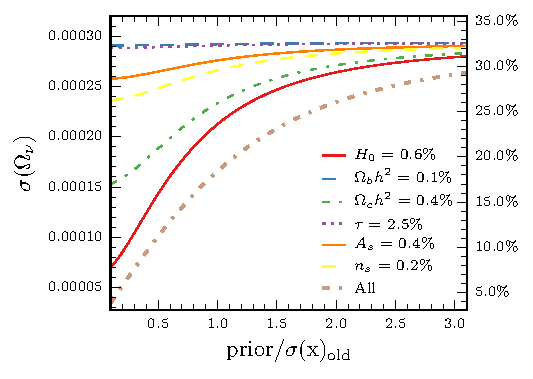
\includegraphics{prior_omnuh2_snow_mass_lmin=4_lmax=4499.pdf}
\caption{$H_{0}$ and $\Omega_{c}h^{2}$ will be the more useful external prior to improve neutrino masses constraint.
In the figure, the constraints on the sum of the neutrino masses as a function of priors on cosmological parameters, as in \reffig{prior_massless_neutrinos} are shown.  Note that constraints would be improved significantly  by distance measurements that constrain $\Omega_ch^2$. We chose a fiducial value $\sum m_{\nu}=85 $ meV.}
\label{fig:prior_omeganuh2}
\end{center}
\end{figure}
%==========

%==========

\begin{figure}[htbp]
\begin{center}
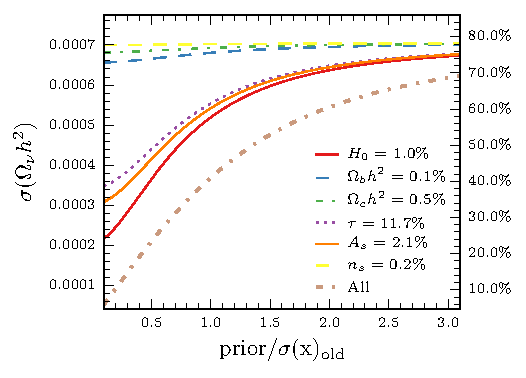
\includegraphics{prior_omnuh2_snow_mass_lmin=50_lmax=3000_ndet=1000000_fsky=0_75.pdf}
\caption{Constraints on the sum of the neutrino masses for $\pmb{\ell_{\rm min}>50}$ as a function of priors on cosmological parameters, as in \reffig{prior_massless_neutrinos}.  Note that constraints would be improved significantly  by distance measurements that constrain $\Omega_ch^2$. The lower limit on the sum of the neutrino masses is 50 meV.}
\label{fig:prior_omeganuh2_tau}
\end{center}
\end{figure}
%==========
As recently pointed out by \cite{allison:2015} there are two important regimes for neutrino masses constraint. In the first one,  large scale are assumed to be accessible by CMB experiments and, as a consequence the optical depth $\tau$ can be constrained internally by measuring the reionization bump. A second possibility is that CMB S4 will be limited to smaller scales and therefore it will have to rely on external priors to constrain $\tau$. This can be given by current stage CMB experiments like Planck as well as future 21 cm survey \cite{liu:2015}. This distinction is important because the optical depth and the neutrino mass are quite degenerate and this will be limiting the constraint in the context of very precise future CMB experiments (see \cite{allison:2015} for details).

\reffig{prior_omeganuh2} shows that, without any external priors, upcoming CMB experiments are poised to obtain 1-sigma limits on $\sum m_\nu$ of order 30 meV, corresponding to close to a 2-sigma detection even in the worst case scenario. Adding in external priors helps this significantly though, as discussed in \cite{2013arXiv1309.5383A,pan:2015,allison:2015}. 
There, the prior was described as ``DESI BAO'', that is a measurement of distances as a function of redshift from the baryon acoustic oscillation feature probed by DESI. Here, the same improvement is parametrized by a strong prior on $\Omega_ch^2$ and $H_{0}$, which indeed determines these low-redshift distances. 
Indeed it is important to keep in mind that a 
As found in \cite{2013arXiv1309.5383A}, the projected error falls below 20 meV with this prior. Adding in other priors would help further.

In \reffig{prior_omeganuh2_tau} we limit CMB accessible modes to $\ell_{\rm min}>50$.


\subsection{Relativistic Degrees of Freedom, $N_{\rm eff}$}

In the standard cosmology, three active neutrinos are thermally produced in the early universe. Were they to decouple well before the epoch of electron-positron annihilation, their energy density after their decoupling would be equal to $3\times (7/8)\times (4/11)^{4/3}\,\rho_{\rm cmb}$, with the first factor capturing the contributions from the 3 active species; the second the difference between fermions and bosons; and the last the relative heating of the photons in the CMB by electron-positron annihilation. However decoupling is not a discrete event and occurs close to the time of electron-positron annihilation, so the neutrinos share a bit in the heating, with the factor of 3 replaced by $N_{\rm eff}=3.046$. The additional fraction depends not only on well-known neutrino scattering rates but also finite temperature quantum corrections. 
Upcoming experiment have the potential to measure this tiny deviation of $N_{\rm eff}$ from 3. This will be an amazing test of our understanding of the Universe when it was about a second old.
Furthermore any possible significant deviation from this value could be a hint of a different scenario not predicted by the standard model. 
%==========
\begin{figure}[htbp]
\begin{center}
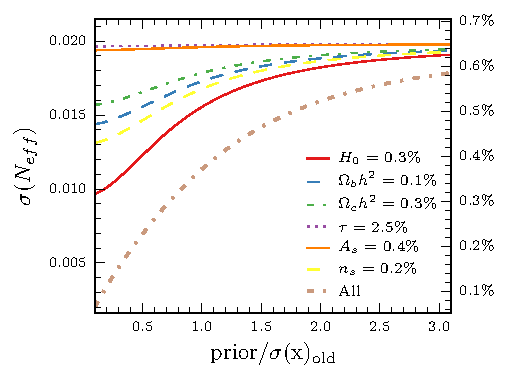
\includegraphics{prior_massless_neutrinos_snow_mass_lmin=4_lmax=4499.pdf}
\caption{Projected 1-sigma error on $N_{\rm eff}$ as a function of the strength of the prior on the other 6 cosmological parameters of the standard $\Lambda$CDM model. Each prior is expressed in units of the error that would be obtained internally from our suite of CMB experiments; e.g., $\sigma(H_0)_{\rm old}=4.1\%$. The parameters that would be most useful to constrain externally for the purposes of determining $N_{\rm eff}$ are $n_s$ and $\Omega_bh^2$. The bottom-most (grey) curve shows the impact of imposing the given prior on {\it all} the other parameters simultaneously.}
\label{fig:prior_massless_neutrinos}
\end{center}
\end{figure}
%==========

\reffig{prior_massless_neutrinos} shows projections for how well our suite of CMB experiments will do at measuring $N_{\rm eff}$ as a function of priors on the other 6 parameters in the standard cosmological model ($H_0, \Omega_mh^2,\Omega_bh^2, n_s, A_s,$ and $\tau$). With no priors on the other parameters, the projected $1$-sigma error is  about $0.02$, suggesting a 2-sigma detection of the deviation from $N_{\rm eff}=3$. The sensitivity comes from the effect of extra species on the damping tail of the CMB anisotropies, both in temperature and polarization, so parameters that also affect the shape of the damping tail, like the slope $n_s$ and the baryon density $\Omega_bh^2$, are most degenerate with $N_{\rm eff}$. As such, \reffig{prior_massless_neutrinos} shows that obtaining external priors on either of these would reduce the errors on $N_{\rm eff}$ to ensure a 3-sigma detection of the partial decoupling prediction. The bottom-most curve shows that if all parameters were constrained externally, then the projected error on $N_{\rm eff}$ would improve significantly.

\subsection{Dark Energy Equation of State, $w$}

While the primordial CMB has limited information about the late-time dark energy equation of state, CMB lensing probes the growth of structure at late times and therefore is sensitive to $w$. Here we are using only the information from the lensing power spectrum as inferred from the CMB, but there is even more information not considered here contained in the many galaxy clusters that upcoming missions will detect via the Sunyaev-Zel'dovich effect. 

%==========

\begin{figure}[htbp]
\begin{center}
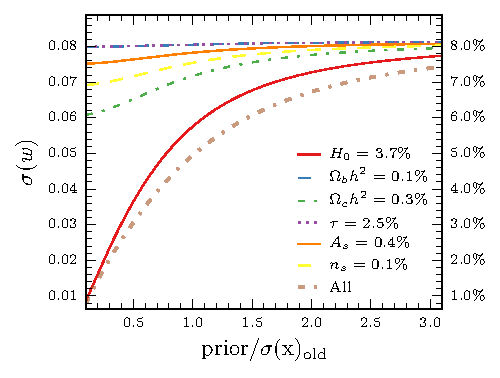
\includegraphics{prior_w_snow_mass_lmin=4_lmax=4499.pdf}
\caption{Constraints on the dark energy equation of state $w$ as a function of priors on cosmological parameters, as in \reffig{prior_massless_neutrinos}. An external prior on $H_{0}$ will be crucial to improve the constraint.} 
\label{fig:prior_w}
\end{center}
\end{figure}
%==========

\reffig{prior_w} shows that without any priors, CMB experiments will not do much better than current constraints, which hover around 10\%. However, an external constraint on the Hubble constant would improve the CMB constraints on $w$ considerably. 
This primarily due to the fact that CMB constrained $w$ through a measurement of the last scattering surface. However that distance can be kept fixed while varying $w$ by accordingly changing the value of $H_{0}$ (and $\Omega_{\Lambda}$ to keep the universe flat). Indeed in a two dimensional ($H_{0},w$) the CMB constrained approximately lies on the constant large scattering surface line.
Notice that an external prior on $H_{0}$ three times more accurate than CMB S4 can improve the CMB constraint almost by a factor of three from a $8\%$ error to a $3\%$ level.

\section{Conclusions  \label{sec:conclusions}}
The planning of the next CMB Stage IV experiments represents an exciting challenge. The possible reward is remarkable. We can finally put a tight constraint on the total mass of neutrinos with deeply implications on particle physics like, for example, the ability to distinguish between normal and inverted hierarchy. We will measure with great accuracy the number of relativistic species, testing both standard model prediction and, eventually, probing new physics. The same is true for dark energy where we will tighten the constraint on $w$,$w_{a}$ getting closer to test the nature of the accelerated expansion of the universe. These however will not be possible without an optimal synergy with other experiments observing a variety of others cosmological probes.
Indeed this should be taken into account in this CMB Stage IV planning phase. Understanding CMB weaknesses and the impact of external data can have a deep influence in planning the experiment specifications.
For this reason in this work we explored the impact of external priors on CMB cosmological constraints and in particular on the neutrino sector and dark energy parameters.
We find:
\begin{description}
\item[$M_{\nu}$] 
\item[$N_{\rm eff}$] 
\item[$w$,$w_{a}$] 
\end{description}

This results suggest...
Comment on issue and future. This will be even more relevant when we open the parameter space. Will CMB + others be able to discover something CMB can't alone? $N_{\rm eff}$ extensions, mass splitting etc




% tables should appear as floats within the text
%
% Here is an example of the general form of a table:
% Fill in the caption in the braces of the \caption{} command. Put the label
% that you will use with \ref{} command in the braces of the \label{} command.
% Insert the column specifiers (l, r, c, d, etc.) in the empty braces of the
% \begin{tabular}{} command.
% The ruledtabular enviroment adds doubled rules to table and sets a
% reasonable default table settings.
% Use the table* environment to get a full-width table in two-column
% Add \usepackage{longtable} and the longtable (or longtable*}
% environment for nicely formatted long tables. Or use the the [H]
% placement option to break a long table (with less control than 
% in longtable).
% \begin{table}%[H] add [H] placement to break table across pages
% \caption{\label{}}
% \begin{ruledtabular}
% \begin{tabular}{}
% Lines of table here ending with \\
% \end{tabular}
% \end{ruledtabular}
% \end{table}

% Surround table environment with turnpage environment for landscape
% table
% \begin{turnpage}
% \begin{table}
% \caption{\label{}}
% \begin{ruledtabular}
% \begin{tabular}{}
% \end{tabular}
% \end{ruledtabular}
% \end{table}
% \end{turnpage}

% Specify following sections are appendices. Use \appendix* if there
% only one appendix.

%\appendix


\begin{acknowledgments}
We thank Youngsoo Park for his contribution in the early stage of this work.
AM wants to thank Zhen Pan who allowed a careful cross-check of our results.
This work was partially supported by the Kavli Institute for Cosmological Physics at the University of Chicago through grants NSF PHY-1125897 and an endowment from the Kavli Foundation and its founder Fred Kavli.
%%%=================================================================
The work of SD is supported by the U.S. Department of Energy, including grant DE-FG02-95ER40896.
\end{acknowledgments}

% Create the reference section using BibTeX:
\bibliography{N_eff_prior_paper}

\end{document}


